\documentclass[journal]{IEEEtran}

% *** CITATION PACKAGES ***
\usepackage{cite}

% *** GRAPHICS RELATED PACKAGES ***
%
\ifCLASSINFOpdf
\usepackage[pdftex]{graphicx}
  % declare the path(s) where your graphic files are
  % \graphicspath{{../pdf/}{../jpeg/}}
  % and their extensions so you won't have to specify these with
  % every instance of \includegraphics
  % \DeclareGraphicsExtensions{.pdf,.jpeg,.png}
\else
  % or other class option (dvipsone, dvipdf, if not using dvips). graphicx
  % will default to the driver specified in the system graphics.cfg if no
  % driver is specified.
  % \usepackage[dvips]{graphicx}
  % declare the path(s) where your graphic files are
  % \graphicspath{{../eps/}}
  % and their extensions so you won't have to specify these with
  % every instance of \includegraphics
  % \DeclareGraphicsExtensions{.eps}
\fi
% graphicx was written by David Carlisle and Sebastian Rahtz. It is
% required if you want graphics, photos, etc. graphicx.sty is already
% installed on most LaTeX systems. The latest version and documentation
% can be obtained at: 
% http://www.ctan.org/pkg/graphicx
% Another good source of documentation is "Using Imported Graphics in
% LaTeX2e" by Keith Reckdahl which can be found at:
% http://www.ctan.org/pkg/epslatex
%
% latex, and pdflatex in dvi mode, support graphics in encapsulated
% postscript (.eps) format. pdflatex in pdf mode supports graphics
% in .pdf, .jpeg, .png and .mps (metapost) formats. Users should ensure
% that all non-photo figures use a vector format (.eps, .pdf, .mps) and
% not a bitmapped formats (.jpeg, .png). The IEEE frowns on bitmapped formats
% which can result in "jaggedy"/blurry rendering of lines and letters as
% well as large increases in file sizes.
%
% You can find documentation about the pdfTeX application at:
% http://www.tug.org/applications/pdftex






% *** PDF, URL AND HYPERLINK PACKAGES ***
%
%\usepackage{url}
% url.sty was written by Donald Arseneau. It provides better support for
% handling and breaking URLs. url.sty is already installed on most LaTeX
% systems. The latest version and documentation can be obtained at:
% http://www.ctan.org/pkg/url
% Basically, \url{my_url_here}.


% correct bad hyphenation here
\hyphenation{op-tical net-works semi-conduc-tor}


\begin{document}
%
% paper title
% Titles are generally capitalized except for words such as a, an, and, as,
% at, but, by, for, in, nor, of, on, or, the, to and up, which are usually
% not capitalized unless they are the first or last word of the title.
% Linebreaks \\ can be used within to get better formatting as desired.
% Do not put math or special symbols in the title.
\title{Análisis Comparativo del Discurso sobre Bitcoin en Redes Sociales y Medios de Noticias}


\author{Álvaro Salgado López}

% note the % following the last \IEEEmembership and also \thanks - 
% these prevent an unwanted space from occurring between the last author name
% and the end of the author line. i.e., if you had this:
% 
% \author{....lastname \thanks{...} \thanks{...} }
%                     ^------------^------------^----Do not want these spaces!
%
% a space would be appended to the last name and could cause every name on that
% line to be shifted left slightly. This is one of those "LaTeX things". For
% instance, "\textbf{A} \textbf{B}" will typeset as "A B" not "AB". To get
% "AB" then you have to do: "\textbf{A}\textbf{B}"
% \thanks is no different in this regard, so shield the last } of each \thanks
% that ends a line with a % and do not let a space in before the next \thanks.
% Spaces after \IEEEmembership other than the last one are OK (and needed) as
% you are supposed to have spaces between the names. For what it is worth,
% this is a minor point as most people would not even notice if the said evil
% space somehow managed to creep in.








% If you want to put a publisher's ID mark on the page you can do it like
% this:
%\IEEEpubid{0000--0000/00\$00.00~\copyright~2015 IEEE}
% Remember, if you use this you must call \IEEEpubidadjcol in the second
% column for its text to clear the IEEEpubid mark.



% use for special paper notices
%\IEEEspecialpapernotice{(Invited Paper)}


\markboth{Procesamiento Y Clasificación de Datos, 16 Enero 2025}{}

% make the title area
\maketitle



%\IEEEpeerreviewmaketitle



\section{Introducción}
% The very first letter is a 2 line initial drop letter followed
% by the rest of the first word in caps.
% 
% form to use if the first word consists of a single letter:
% \IEEEPARstart{A}{demo} file is ....
% 
% form to use if you need the single drop letter followed by
% normal text (unknown if ever used by the IEEE):
% \IEEEPARstart{A}{}demo file is ....
% 
% Some journals put the first two words in caps:
% \IEEEPARstart{T}{his demo} file is ....
% 
% Here we have the typical use of a "T" for an initial drop letter
% and "HIS" in caps to complete the first word.
\IEEEPARstart
{B}{i} tcoin, como criptomoneda pionera, ha generado un gran interés a nivel mundial, tanto por su potencial disruptivo en los sistemas financieros como por su alta volatilidad. Las reacciones y percepciones sobre Bitcoin en diferentes plataformas reflejan de manera directa las expectativas y opiniones de la sociedad respecto a su futuro y desempeño. Analizar estas percepciones puede ofrecer información valiosa sobre las tendencias y factores que afectan su valor y adopción.

El análisis de sentimientos aplicado a plataformas de redes sociales y medios de comunicación permite explorar cómo se sienten los usuarios y las audiencias ante temas específicos. En este estudio, se realiza un análisis comparativo de los sentimientos expresados sobre Bitcoin en dos fuentes clave: Twitter y NewsAPI.

Twitter, por ser una plataforma de microblogging ampliamente utilizada, es conocida por sus reacciones rápidas y a menudo emocionales sobre eventos de actualidad. Los usuarios de Twitter tienden a compartir opiniones breves sobre temas como Bitcoin, lo que genera una gran cantidad de datos que reflejan tanto la especulación como las reacciones a noticias y movimientos del mercado.

Por otro lado, NewsAPI proporciona acceso a noticias de una amplia gama de fuentes, que incluyen medios establecidos como Reuters, Forbes y CNN, lo que ofrece una perspectiva más formal y estructurada sobre Bitcoin. Las noticias extraídas a través de esta API incluyen tanto reportes de eventos recientes como análisis más profundos sobre el mercado y su contexto económico.

El objetivo de este análisis es comparar los sentimientos expresados en Twitter y en las noticias de NewsAPI sobre Bitcoin, identificando las emociones predominantes y las diferencias entre las reacciones de los usuarios en redes sociales frente a los enfoques más tradicionales y académicos de los medios de comunicación. Para ello, se utilizaron técnicas de procesamiento de lenguaje natural (PLN) para evaluar los sentimientos en ambas fuentes, categorizando los resultados en positivos, negativos y neutrales.
% You must have at least 2 lines in the paragraph with the drop letter
% (should never be an issue)

\section{Resultados}
\subsection{Frecuencia de palabras más comunes}

El análisis de las palabras más frecuentes en Twitter reveló un enfoque claro en temas de interés inmediato y relacionados con la especulación del mercado. Esto es consistente con la naturaleza de esta red social, donde los usuarios tienden a discutir sobre eventos recientes, fluctuaciones de precios y estrategias rápidas. Las palabras más mencionadas fueron:
\begin{itemize}
    \item Target: 45 menciones. Indicativo de metas o niveles de precios esperados por los usuarios.
    \item High: 26 menciones. Relacionado con máximos de precios o expectativas de incrementos en el valor de Bitcoin.
    \item New: 24 menciones. Refleja la discusión sobre novedades o desarrollos recientes en el ecosistema de Bitcoin.
    \item BTC: 21 menciones. Representa el símbolo de Bitcoin, usado frecuentemente para referirse a la criptomoneda en términos técnicos.
    \item Price: 21 menciones. Evidencia el interés de los usuarios en las fluctuaciones del precio de Bitcoin.
\end{itemize}
La predominancia de estas palabras sugiere que los usuarios de Twitter tienen un enfoque especulativo y táctico, priorizando temas relacionados con la dinámica diaria del mercado.

Por otro lado, el análisis de las palabras más frecuentes en los artículos de noticias recopilados a través de NewsAPI reflejó un enfoque más amplio y técnico. Las palabras más comunes fueron:
\begin{itemize}
    \item Bitcoin: 39 menciones. Refleja el tema central de los artículos, abordado desde diversas perspectivas como mercado, regulación y adopción.
    \item Crypto: 20 menciones. Representa el término genérico para criptomonedas, indicando que el contexto no se limita exclusivamente a Bitcoin.
    \item XRP: 10 menciones. Denota interés en otras criptomonedas destacadas, mostrando diversidad en los enfoques de las noticias.
    \item ETFs: 9 menciones. Refleja la discusión sobre fondos cotizados en bolsa relacionados con Bitcoin, un tema recurrente en el ámbito financiero.
    \item Price: 8 menciones. Evidencia un interés compartido con Twitter sobre el valor de mercado de Bitcoin, aunque desde un ángulo más analítico.
\end{itemize}
El enfoque en NewsAPI está claramente orientado hacia análisis financieros, regulaciones y desarrollos tecnológicos en el ecosistema cripto, lo que contrasta con la conversación más especulativa en Twitter.

El análisis de sentimientos aplicado a los textos extraídos de Twitter mostró una predominancia del sentimiento positivo en las discusiones sobre Bitcoin, como se muestra en la Fig \ref{twitter} Esto refleja un estado de ánimo optimista y entusiasta por parte de los usuarios.
\begin{figure}
    \centering
    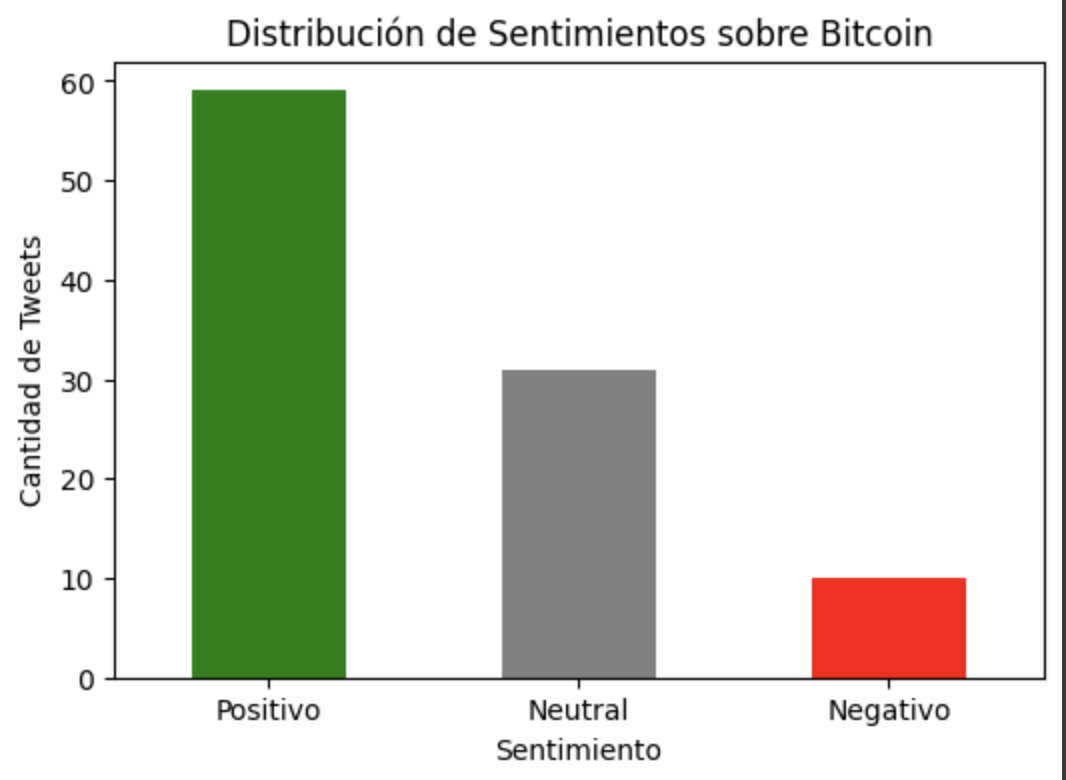
\includegraphics[width=0.5\linewidth]{Figs/Twitter.png}
    \caption{Análisis de sentimientos en Twitter}
    \label{twitter}
\end{figure}

Este hallazgo es consistente con la naturaleza de Twitter, una plataforma donde los usuarios suelen expresar emociones fuertes y opiniones polarizadas, frecuentemente inclinadas hacia el optimismo en temas de interés.

En contraste, los artículos recopilados de NewsAPI presentaron mayormente un sentimiento neutro mostrado en la Fig \ref{newsapi}, lo que refleja un enfoque objetivo y técnico por parte de las fuentes periodísticas. 

La neutralidad observada es típica en los medios de comunicación, especialmente cuando cubren temas financieros y tecnológicos de impacto global.
\begin{figure}
    \centering
    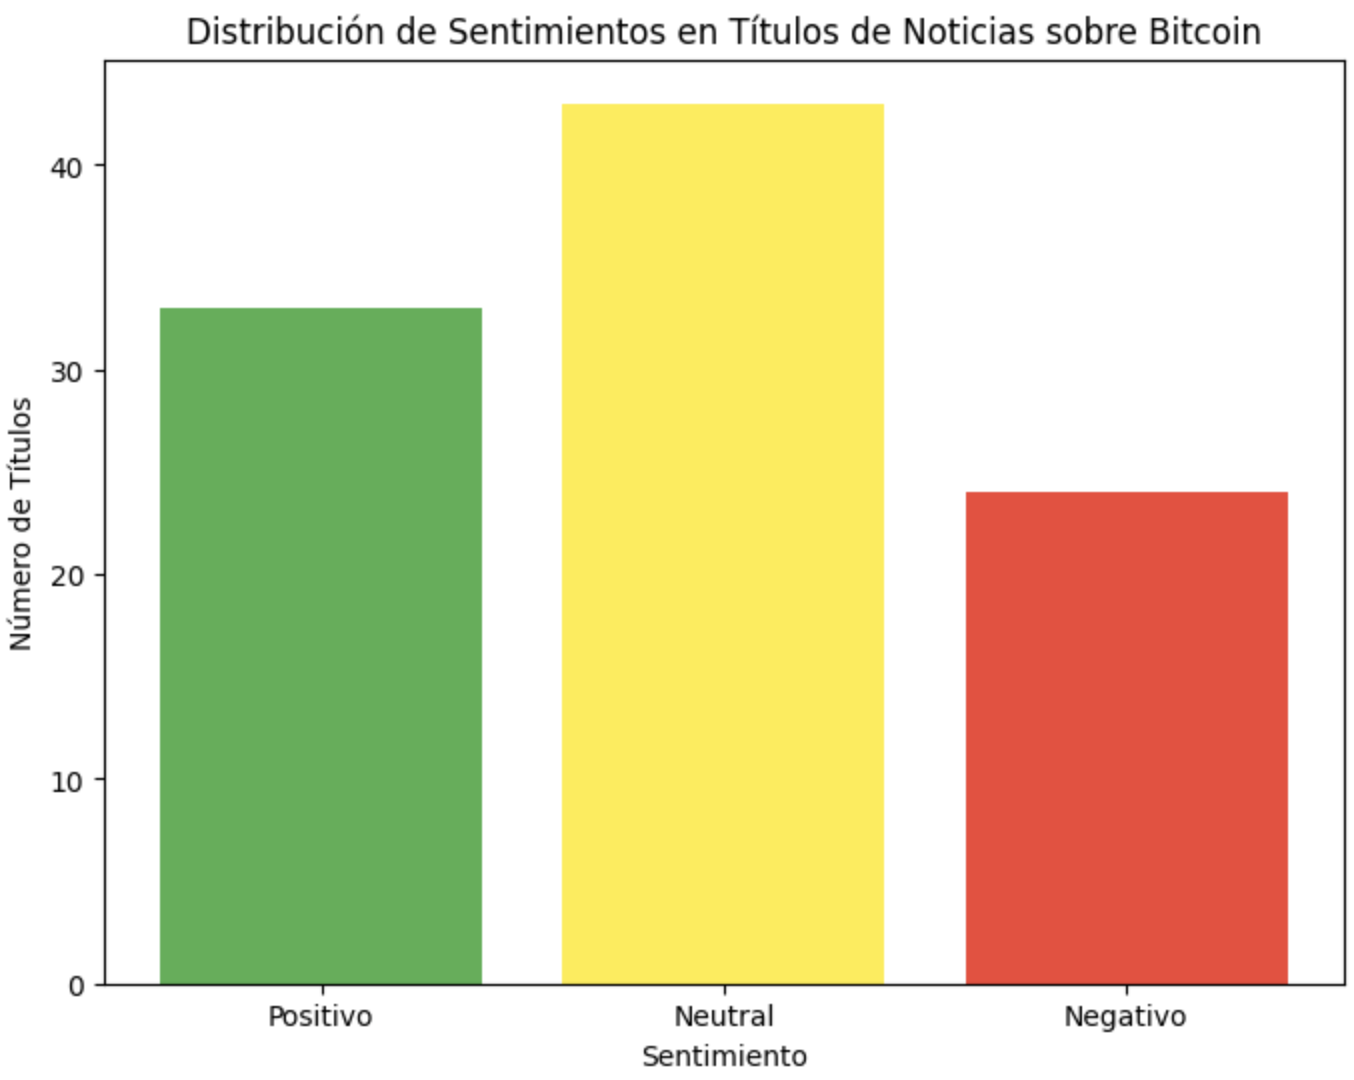
\includegraphics[width=0.5\linewidth]{Figs/NewsAPI.png}
    \caption{Análisis de sentimientos en NewsAPI}
    \label{newsapi}
\end{figure}

\section{Conclusión}
El análisis comparativo entre Twitter y las noticias obtenidas a través de NewsAPI ofrece una perspectiva valiosa sobre cómo se discute Bitcoin en diferentes contextos.

Twitter se caracteriza por un discurso centrado en movimientos especulativos y oportunidades inmediatas de mercado. Las palabras más frecuentes, como “target”, “high” y “price”, reflejan un interés en proyecciones y estrategias de corto plazo, impulsadas por la interacción directa entre los usuarios. Este enfoque está acompañado de un tono optimista, como lo evidencia el predominio de sentimientos positivos en los textos analizados.

Las noticias obtenidas mediante NewsAPI, en cambio, adoptan un enfoque técnico y amplio, abarcando temas como regulaciones, análisis de mercado y el papel de otras criptomonedas. Las palabras más comunes, como “bitcoin”, “crypto” y “ETFs”, sugieren un análisis profundo y multifacético del ecosistema cripto. La preponderancia de sentimientos neutros resalta la intención de los medios de ofrecer información objetiva y contextualizada.

Los usuarios de Twitter tienden a expresar emociones y opiniones marcadas, lo que podría influir en la percepción general de Bitcoin como una oportunidad atractiva y positiva. Este comportamiento es consistente con el diseño de la plataforma, que fomenta la interacción rápida y emocional.
Las fuentes de noticias, en contraste, presentan un tono moderado y fundamentado, alineado con la expectativa de profesionalismo y precisión en el ámbito periodístico.

Los resultados demuestran que el discurso sobre Bitcoin es heterogéneo y depende del canal en el que se desarrolle. Mientras que las redes sociales fomentan una narrativa impulsiva y cargada de expectativas, los medios de comunicación promueven un entendimiento más equilibrado y analítico.

Este contraste subraya la importancia de considerar múltiples fuentes para obtener una visión completa del tema, especialmente en un campo tan dinámico y polarizado como el de las criptomonedas.

En síntesis, este estudio resalta cómo las plataformas digitales moldean la narrativa sobre Bitcoin de maneras diferentes, influyendo en la percepción pública y profesional de esta tecnología. Esto refuerza la necesidad de un análisis crítico y diversificado al abordar temas de alto impacto como las criptomonedas.


% Can use something like this to put references on a page
% by themselves when using endfloat and the captionsoff option.
\ifCLASSOPTIONcaptionsoff
  \newpage
\fi



% trigger a \newpage just before the given reference
% number - used to balance the columns on the last page
% adjust value as needed - may need to be readjusted if
% the document is modified later
%\IEEEtriggeratref{8}
% The "triggered" command can be changed if desired:
%\IEEEtriggercmd{\enlargethispage{-5in}}

% references section

% can use a bibliography generated by BibTeX as a .bbl file
% BibTeX documentation can be easily obtained at:
% http://mirror.ctan.org/biblio/bibtex/contrib/doc/
% The IEEEtran BibTeX style support page is at:
% http://www.michaelshell.org/tex/ieeetran/bibtex/
%\bibliographystyle{IEEEtran}
% argument is your BibTeX string definitions and bibliography database(s)
%\bibliography{IEEEabrv,../bib/paper}
%
% <OR> manually copy in the resultant .bbl file
% set second argument of \begin to the number of references
% (used to reserve space for the reference number labels box)

%\bibliographystyle{IEEEtran} % Estilo de citas de IEEE
%\bibliography{referencias} % Nombre de tu archivo .bib


\end{document}


